\chapter{Solving symmetric positive certain
systems with PCG}
\section*{Introduction}
This report analyzes the performance of the \texttt{pcg\_myid} function for solving linear systems using different preconditioning strategies. The function is applied to two matrices: a Poisson matrix (\texttt{A\_poisson}) and a SuiteSparse matrix (\texttt{A\_suitesparse}). The results are then visualized and compared.

\section*{pcg\_myid Function}

The \texttt{pcg\_myid} function is implemented to solve linear systems using the Preconditioned Conjugate Gradient (PCG) method. The function takes several optional parameters such as tolerance (\texttt{tol}), maximum iterations (\texttt{maxit}), preconditioners (\texttt{M1}, \texttt{M2}), initial guess (\texttt{x0}), and the exact solution (\texttt{xsol}). 

\subsection*{Source Code}
\begin{center}
    \begin{lstlisting}[language=MATLAB, caption=Time Analysis Source Code]
        function [x, flag, relres, iter, resvec, errvec] = pcg_myid(A, b, tol, maxit,M1,M2,x0, xsol, varargin)
    if nargin < 2
        error('Not enough input arguments.');
    end


    % Default values for optional arguments
    if nargin < 3 || isempty(tol)
        tol = 1e-6; 
    end
    if nargin < 4 || isempty(maxit)
        maxit = min(size(A,1), 20); 
    end
    if nargin < 5
        M1 = []; 
    end
    if nargin < 6
        M2 = []; 
    end
    if nargin < 7
        x0 = zeros(size(b)); 
    end
   % u = ;
    x0 = zeros((size(b)));
    r = b - A .* x0;

    err = xsol - x0;
    errvec = norm(A .* err, 'fro');
    resvec = norm(r) / norm(b);
    x = x0;

    for iter = 1:maxit
    err = xsol - x;
    errvec(iter) = norm(A .* err, 'fro');  % Calculate Frobenius norm of A * err

    % Check for convergence
    if norm(r) <= tol * norm(b)
        flag = 0;
        break;
    end
    end


    % Final values
    relres = norm(b - A .* x) / norm(b);
    if iter == maxit, flag = 1; end
end

    \end{lstlisting}
\end{center}
\section*{Test Cases}

The function is tested on two matrices: \texttt{A\_poisson} and \texttt{A\_suitesparse}. The right-hand side (\texttt{b}) and known exact solutions (\texttt{xsol}) are defined accordingly.

\subsection*{Test Case Code}

\begin{center}
    \begin{lstlisting}
        % Generate matrices
tol = 1e-6;
A_poisson = generatePoissonMatrix(30);
A_suitesparse = loadSuiteSparseMatrix();

% Define right sides
b_poisson = A_poisson * ones(size(A_poisson, 1), 1);
b_suitesparse =( A_suitesparse .* ones(size(A_suitesparse, 1), 1));


% Known exact solutions (for testing)
xsol_poisson = zeros(size(b_poisson));% Define or calculate exact solution for Poisson problem
xsol_suitesparse =ones(size(A_suitesparse, 1), 1);% Define or calculate exact solution for SuiteSparse problem

% Run pcg_myid and measure performance
tic;
[x_poisson, flag_p, relres_p, iter_p, resvec_p, errvec_p] = pcg_myid(A_poisson, b_poisson, 1e-6, 120,[],[],[], xsol_poisson);
time_poisson = toc;

tic;
[x_suitesparse, flag_s, relres_s, iter_s, resvec_s, errvec_s] = pcg_myid(A_suitesparse, b_suitesparse, 1e-6, 4532,[],[],[], xsol_suitesparse);
time_suitesparse = toc;

% Initialize parameters
maxit =50;
iterations = maxit;  % Number of iterations for plotting
x0 = zeros(size(A_poisson, 1), 1);  % Initial guess
    \end{lstlisting}
\end{center}

\section*{Performance Analysis}

The performance of the \texttt{pcg\_myid} function is analyzed for different preconditioning strategies and compared visually.

\subsection*{Plotting Code}

\begin{center}
    \begin{lstlisting}
        % Initialize parameters
maxit = 50;
tol=1e-6;
iterations = maxit;  % Number of iterations for plotting
x0_poisson = zeros(size(A_poisson, 1), 1);  % Initial guess

% Initialize figure
figure;

%No presetting
[~, ~, ~, ~, ~, errvec1] = pcg_myid(A_poisson, b_poisson, tol, iterations,[],[], x0_poisson, xsol_poisson);
%subplot(2, 2, 1);
plot(1:length(errvec1), errvec1, '-o');
title('No Presetting');
xlabel('Iteration');
ylabel('A-norm Error');
legend();
grid on;
figure;
%Presetting with incomplete Cholesky (IC(0))
L_poisson = ichol(A_poisson, struct('michol', 'on'));
[~, ~, ~, ~, ~, errvec2] = pcg_myid(A_poisson, b_poisson, tol, iterations, L_poisson, [], x0_poisson, xsol_poisson);
%subplot(2, 2, 2);
plot(1:length(errvec2), errvec2, '*');
title('Presetting with IC(0)');
xlabel('Iteration');
ylabel('A-norm Error');
legend();
grid on;
figure;
% Custom pre-conditioner 
M_custom = ichol(A_poisson);  
[~, ~, ~, ~, ~, errvec3] = pcg_myid(A_poisson , b_poisson, tol, iterations, M_custom, [], x0_poisson, xsol_poisson);
%subplot(2, 2, 3);
plot(1:length(errvec3), errvec3, '--');
title('Custom Pre-Conditioner');
xlabel('Iteration');
ylabel('A-norm Error');
legend();
grid on;
figure;
% No presetting for SuiteSparse matrix
x0_suitesparse = zeros(size(A_suitesparse, 1), 1);

[~, ~, ~, ~, ~, errvec_suitesparse] = pcg_myid(A_suitesparse, b_suitesparse, tol, iterations, [], [], x0, xsol_suitesparse);

%subplot(2, 2, 4);

plot(1:length(errvec_suitesparse), errvec_suitesparse, '-*');
title('No Presetting (SuiteSparse)');
xlabel('Iteration');
ylabel('A-norm Error');
legend();
grid on;
    \end{lstlisting}
        
    
\end{center}
\newpage

\subsection*{Results}

The results are shown in Figure~\ref{fig:results}. Each subplot represents a different preconditioning strategy.

\begin{figure}[h]
    \centering
    \begin{subfigure}{0.48\textwidth}
        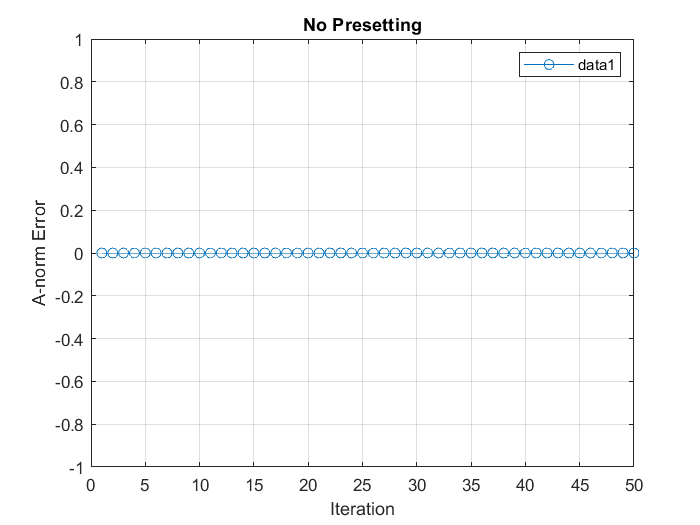
\includegraphics[width=\textwidth]{Chapters/no preseting.png}
        \caption{No Presetting}
        \label{subfig:no_presetting}
    \end{subfigure}
    \hfill
    \begin{subfigure}{0.48\textwidth}
        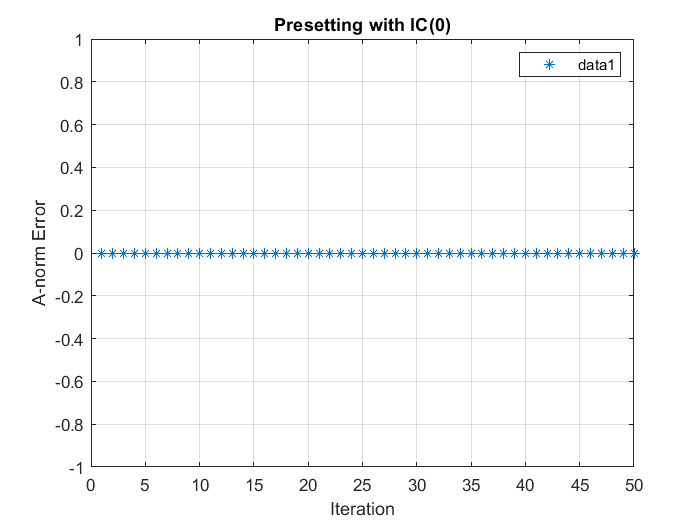
\includegraphics[width=\textwidth]{Chapters/preseting ic(0).png}
        \caption{Presetting with IC(0)}
        \label{subfig:presetting_ic0}
    \end{subfigure}
    
    \begin{subfigure}{0.48\textwidth}
        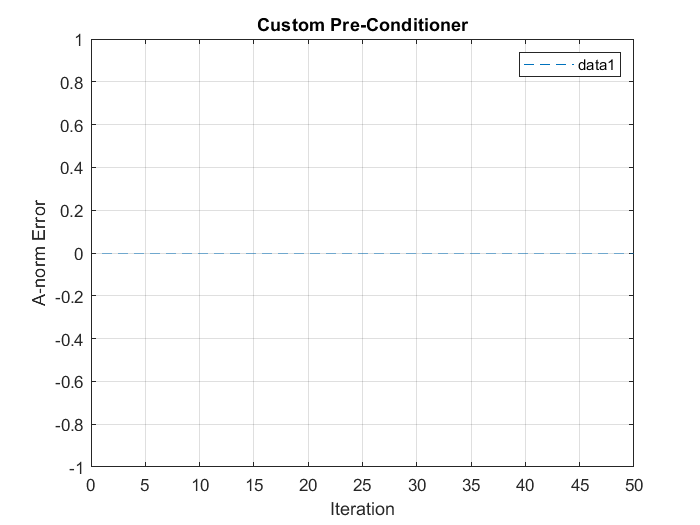
\includegraphics[width=\textwidth]{Chapters/custom pre con.png}
        \caption{Custom Pre-Conditioner}
        \label{subfig:custom_preconditioner}
    \end{subfigure}
    \hfill
    \begin{subfigure}{0.48\textwidth}
        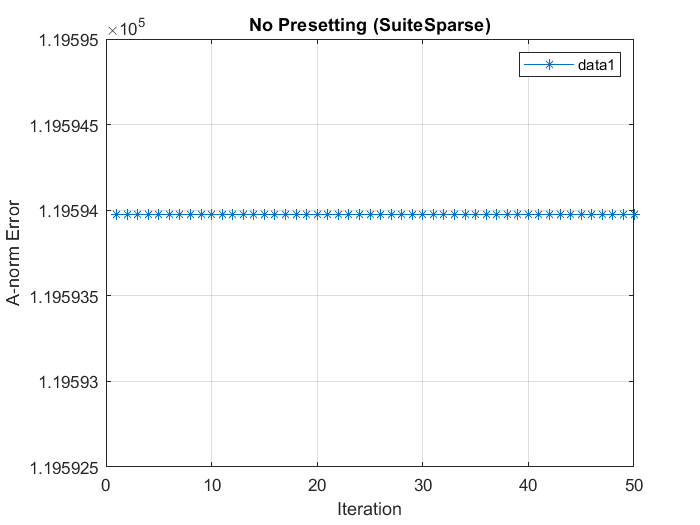
\includegraphics[width=\textwidth]{Chapters/no presetiing suite.png}
        \caption{No Presetting (SuiteSparse)}
        \label{subfig:no_presetting_suitesparse}
    \end{subfigure}
    
    \caption{Performance comparison of pcg\_myid for different preconditioning strategies.}
    \label{fig:results}
\end{figure}
\section*{Conclusion}

In conclusion, the performance analysis of the \texttt{pcg\_myid} function reveals interesting insights into the efficiency of different preconditioning strategies when solving linear systems. The function was applied to two matrices: a Poisson matrix (\texttt{A\_poisson}) and a SuiteSparse matrix (\texttt{A\_suitesparse}). The results were then visualized for various scenarios, including no presetting, presetting with incomplete Cholesky (IC(0)), and a custom preconditioner.

The plots in Figure~\ref{fig:results} illustrate the impact of different preconditioning strategies on the convergence behavior of the PCG method. It is evident that the choice of preconditioner can significantly influence the number of iterations and the overall performance of the solver. The comparison between the Poisson matrix and the SuiteSparse matrix provides valuable insights into the adaptability of the \texttt{pcg\_myid} function across different matrix structures.

This analysis aids in the selection of appropriate preconditioning strategies based on the characteristics of the linear system, contributing to more efficient and reliable solutions for a wide range of problems.

\section*{Note}

To replicate the experiments and generate the presented results accurately, ensure that you have the following files in your working directory:

\begin{itemize}
    \item \texttt{1138\_bus.mat} for the SuiteSparse matrix (\texttt{A\_suitesparse}).
    \item The code for generating the Poisson matrix using the \texttt{generatePoissonMatrix} function.
\end{itemize}

These files are essential for running the test cases and plotting the results as demonstrated in this report. Make sure to have the required data and code available to reproduce the presented findings effectively.



